\documentclass[a4paper, 12pt]{article}

\usepackage{IEEEtrantools}
\usepackage[]{amsmath}
\usepackage{amssymb}
\usepackage{float}
\usepackage[]{graphicx}
\usepackage{subfig}
\usepackage{caption}


\title{Control Systems 4A Practical 2 Report}
\author{216054484 \and 216008466}

\begin{document}

\pagenumbering{gobble}
\begin{titlepage}
  \maketitle
\end{titlepage}

\pagenumbering{roman}
\tableofcontents
\newpage
\pagenumbering{arabic}

\section{Question 1} % (fold)
\label{sec:question_1}
Using the student number 216008466 gives the masses for this question to be $M = 2.8$kg, $m = 0.16$kg and the distance betweent the rod and the mass to be $3.5$

\subsection{Implementing the Linear State-space Model} % (fold)
\label{sub:implementing_the_linear_state_space_model}
The system implemented  using the student number as previously stated gives the state-space model as follows 
\begin{equation}
  A = \left[
  \begin{array}{c c c c}
   	0 & 1 & 0 & 0 \\
   	0.302 &  0 & 0 & 0\\
   	0 & 0 & 0 & 1\\
   	-0.56 &  0 &  0 &  0\\
  \end{array}
  \right]
  \label{eq:a_q1}
\end{equation}

\begin{equation}
  B = \left[
  \begin{array}{c}
   0 \\-\frac{5}{59}\\ 0\\\frac{1}{2.8}
  \end{array}
  \right]
  \label{eq:b_q1}
\end{equation}

\begin{equation}
  C = \left[
  \begin{array}{c c c c}
    1 & 0 & 0 & 0\\
    0 & 0 & 1 & 0\\
  \end{array}
  \right]
  \label{eq:c_q1}
\end{equation}


% subsection implementing_the_linear_state_space_model (end)

\subsection{Full State Feedback System} % (fold)
\label{sub:full_state_feedback_system}
A series of steps need to followed in order to realize control for this system, we start off with finding the control law as defined by equation \eqref{eq:control_law}
\begin{equation}
  u = -\left[
  \begin{array}{cccc}
    K1&K2&...&Kn
  \end{array}
  \right]
  \left[
  \begin{array}{c}
    x_1 \\
    x_2\\
    ...\\
    x_n
  \end{array}
  \right]
  \label{eq:control_law}
\end{equation}

\eqref{eq:control_law} tells us that the system has a constant matrix in the feedback path. For an $n^{th}$ order system there are $n$ feedback gains. The pole locations of the system can be set using the appropriate values  of $K_1, ... , K_n$ in the closed loop characteristic equation given as $det[s\textbf{I}-(\textbf{A}-\textbf{BK})] = 0$. Thus our design narrows down to finding the values of $K_i$ such that the system poles are placed in the locations as specified by the question, to do this we must first find the desired pole locations by doing something something and another something <+PROCEDURE FOR FINDING THE POLES MUST BE DISCUSSED HERE+>\\

After calculating the pole locations based on the required settling time and percent overshoot of $1.5$s and $20\%$, we use the \texttt{place} octave command which has a better accuracy than the \texttt{acker} command (it must be noted that the place command can only be applied if the desired poles are distinct which in this case is <+OR IS NOT WE HAVE TO CALCULATE THE POLES TO MAKE THIS STATEMENT+>). This gives us the control law needed to place the system in the desired pole locations.\\

Using these constant values we can now obtain the controlled matrix defined by the equation $A_{controlled} = \textbf{A}-\textbf{B}\textbf{K};$. The Octave code that implements all of this is shown below

\noindent
	\texttt{A = [0 1 0 0;0.302 0 0 0;0 0 0 1;-0.56 0 0 0];}\\
	\texttt{B = [0 ;-5/59; 0; 1/2.8];}\\
	\texttt{C = [1 0 0 0;0 0 1 0];}\\
	\texttt{sys = ss(A,B,C);}\\
	\texttt{step(sys);}\\
	\texttt{[num,den] = ss2tf(A,B,C);}\\
	\texttt{transfer = tf(num,den);}\\
	\texttt{figure;}\\
	\texttt{pzmap(transfer);}\\
	\texttt{P = eig(A)}\\
	\texttt{OS = 0.2;}\\
	\texttt{ts = 1.5;}\\
	\texttt{zeta = (-log(OS))/(sqrt(pi\^2 + (log(OS))\^2));}\\
	\texttt{wn = 4.6/(ts\*zeta);}\\
	\texttt{sigma = zeta * wn;}\\
	\texttt{wd = sqrt(wn\^2 - sigma\^2);}\\
	\texttt{p1 = (-sigma + wd\*i);}\\
	\texttt{p2 = 1.382\*(-sigma);}\\
	\texttt{p3 = (-sigma - wd*i);}\\
	\texttt{p4 = 1.382\*(-sigma);}\\
	\texttt{poles\_desired = [p1 p2 p3 p4];}\\
	\texttt{K = acker(A,B,poles\_desired);}\\
	\texttt{A\_controlled = A-B\*K;}\\
	\texttt{System\_controlled = ss(A\_controlled,B,C);}\\
	\texttt{figure;}\\
	\texttt{step(System\_controlled);}\\

\newpage
Where the desired pole locations were calculated using the formula $s_{1,2} =\zeta \omega_n \pm j\omega_n\sqrt{\zeta^2-1}$ and $\omega$, $t_s = \frac{4}{\omega_n}$ and $\zeta = \frac{-\log(OS)}{\sqrt{\pi^2+\log^2(OS)}}$. The results of running this code follows 

\begin{figure}[H]
  \centering
  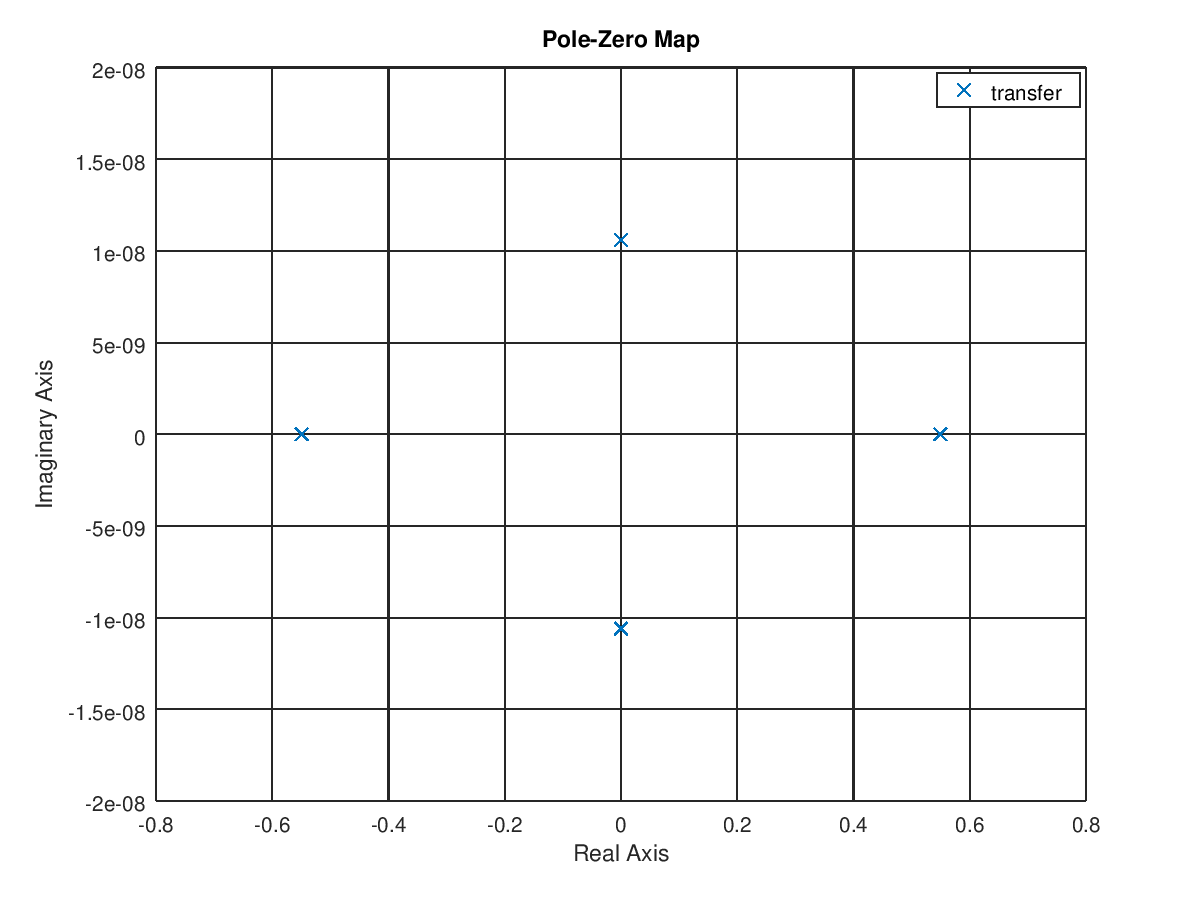
\includegraphics[width=\textwidth]{images/pzmap.png}
  \caption{Pole zero map of the system with no control showing a pole in the right half plane giving rise to an unstable system}
  \label{fig:pzmap}
\end{figure}

\begin{figure}[H]
  \centering
  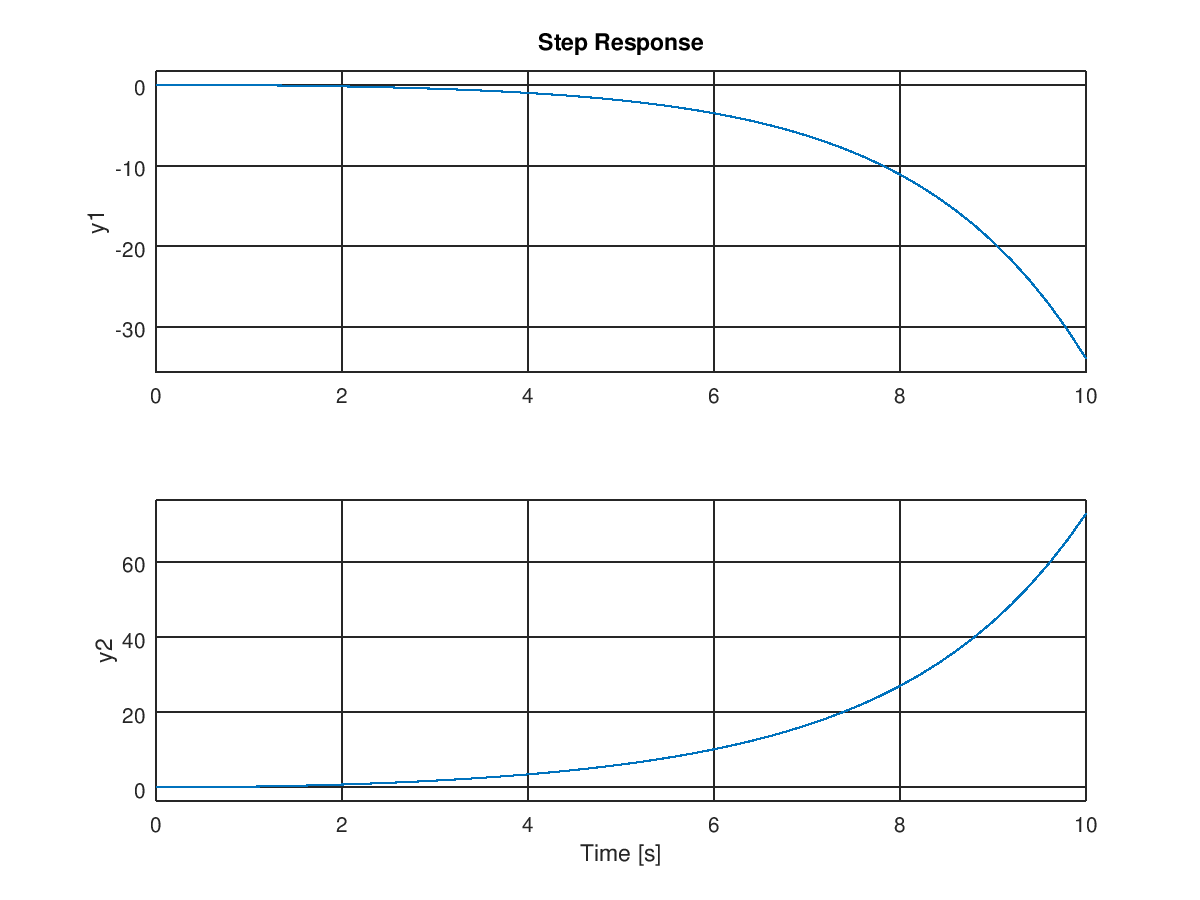
\includegraphics[width=\textwidth]{images/nocontrol.png}
  \caption{Step response of the state space representation of the system with no control implemented, showing an unstable system as alluded to by the pzmap of Figure \ref{fig:pzmap}}
  \label{fig:nocontrol}
\end{figure}

\begin{figure}[H]
  \centering
  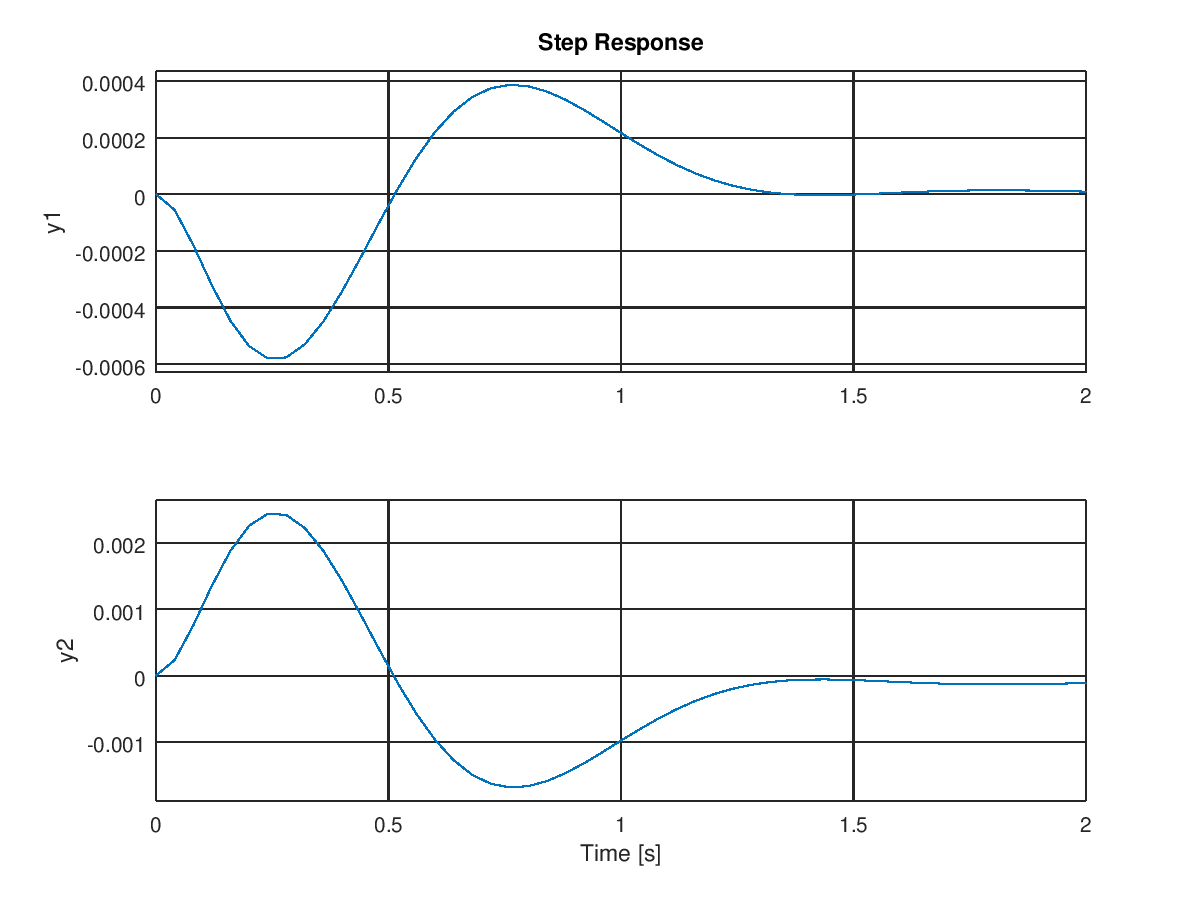
\includegraphics[width=\textwidth]{images/control.png}
  \caption{Control law implemented on the unstable system, the poles in the right half plane were moved according to the code discussed previously}
  \label{fig:control}
\end{figure}

Figure \ref{fig:control} shows that we have effectively implemented feedback control for the system. From Figure \ref{fig:control} we see the output \texttt{y1} approaches $0$, the expected result for the pendulum to stay upright. From the plot we ca also see that the overshoot and the settling time is within the design for specification of respectively $20\%$ and $1.5$s



% subsection full_state_feedback_system (end)

% section question_1 (end)

\section{Question 2}

In this question, we consider the following circuit:

\begin{figure}[H]
  \centering
  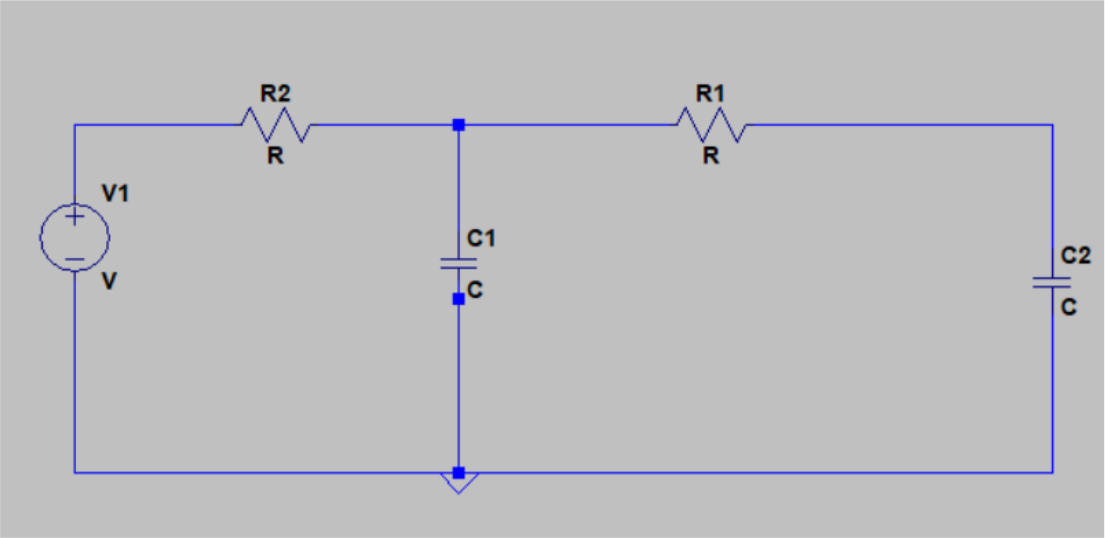
\includegraphics[width=.8\textwidth]{./images/circuit.png}
  \caption{}
  \label{fig:circuit}
\end{figure}

\subsection{State-space Representation}

In order to find the general state-space equations of this circuit, we start
with a few preliminary equations.

\begin{equation}
  i_{C1} = C_1 \dot{V_{C1}}
  \label{eq:ic1}
\end{equation}

\begin{equation}
  i_{C2} = C_2 \dot{V_{C2}}
  \label{eq:ic2}
\end{equation}

Then, we use Kirchoff's current law to get the following equation:

\begin{IEEEeqnarray}{rCl}
  i_1 & = & i_{C1} + i_{C2} \nonumber \\
  & = & C_1 \dot{V_{C1}} + C_2 \dot{V_{C2}}
  \label{eq:kcl}
\end{IEEEeqnarray}

Using Kirchoff's Voltage law at the right-most loop, and substituting from
\eqref{eq:kcl}, we get

\begin{IEEEeqnarray}{rCl}
  V_{C1} & = & V_{R2} + V_{C2} \nonumber \\
  & = & i_{C2}R_2 + V_{C2} \nonumber \\
  & = & R_2 C_2 \dot{V}_{C2} + V_{C2} \nonumber \\
  R_2 C_2 \dot{V}_{C2} & = & V_{C1} - V_{C2} \nonumber \\
  \dot{V}_{C2} & = & \frac{1}{R_2 C_2} V_{C1} - \frac{1}{R_2 C_2} V_{C2}
  \label{eq:kvl2}
\end{IEEEeqnarray}

Then, using the results from \eqref{eq:kcl} and \eqref{eq:kvl2}, and performing
Kirchoff's Voltage Law at the loop with the input voltage, we get

\begin{IEEEeqnarray}{rCl}
  V_i & = & V_{R1} + V_{C1} \nonumber \\
  & = & i_1 R_1 + V_{C1} \nonumber \\
  & = & R_1 \left[ C_1 \dot{V}_{C1} + C_2 \dot{V}_{C2} \right] + V_{C1} \nonumber \\
  & = & R_1 C_1 \dot{V}_{C1} + R_1 C_2 \dot{V}_{C2} + V_{C1} \nonumber \\
  & = & R_1 C_1 \dot{V}_{C1} + R_1 C_2 \left( \frac{1}{R_2 C_2} V_{C1} - \frac{1}{R_2 C_2} V_{C2} \right) + V_{C1} \nonumber \\
  R_1 C_1 \dot{V}_{C1} & = & - \left( \frac{R_1 + R_2}{R_2} \right) V_{C1} +  \frac{R_1}{R_2} V_{C2} + V_i \nonumber \\
  \dot{V}_{C1} & = & -\frac{R_1 + R_2}{R_1 R_2 C_1} V_{C1} + \frac{1}{R_2 C_1} V_{C2} + \frac{1}{R_1 C_1} V_i
\end{IEEEeqnarray}

This leaves us with the following state-space matrices:

\begin{equation}
  A = \left[
  \begin{array}{cc}
    -\frac{R_1 + R_2}{R_1 R_2 C_1} & \frac{1}{R_2 C_1} \\
    \frac{1}{R_2 C_2} & -\frac{1}{R_2 C_2}
  \end{array}
  \right]
  \label{eq:ss_A}
\end{equation}

\begin{equation}
  B = \left[
  \begin{array}{c}
    \frac{1}{R_1 C_1} \\
    0
  \end{array}
  \right]
  \label{eq:ss_B}
\end{equation}

Assuming that we take our output across capacitor $C_2$, we have

\begin{equation}
  C = \left[
  \begin{array}{c c}
    0 & 1
  \end{array}
  \right]
  \label{eq:ss_C}
\end{equation}

and finally,

\begin{equation}
  D = \left[ 0 \right]
  \label{eq:ss_D}
\end{equation}

On the question of stability, we can easily deduce that the system is stable by
applying the operating principles of a capacitor to the problem. A capacitor
can only store a certain maximum amount of charge, at which point, if it has no
path in which to discharge, it will theoretically hold this charge forever. The
stability of a system is defined in the value it settles on when $t \rightarrow
\infty$. In the case of our circuit, when $t$ does approach infinity, $C2$ and
$C1$ will be fully charged, the voltage across them would be $V_i$, and no
current would flow in the circuit unless a load is connected over $C2$ so that
the capacitors can discharge. Therefore, this circuit is always stable.

\subsection{Controllability and Observability}

Let us take the following values for our components: $R_1 = R_2 = 50\Omega$,
$C_1 = 3.9 \mu F$, $C_2 = 4.7 \mu F$. Then we have

\begin{equation}
  A = \left[
  \begin{array}{cc}
    -1.03 \times 10^4 & 5.13 \times 10^3 \\
    4.26 \times 10^3 & -4.26 \times 10^3
  \end{array}
  \right]
  \label{eq:q_A}
\end{equation}

\noindent and

\begin{equation}
  B = \left[
  \begin{array}{c}
    5.13 \times 10^3 \\
    0
  \end{array}
  \right]
  \label{eq:q_B}
\end{equation}

Then we have controllability matrix

\begin{equation}
  C_M = \left[
  \begin{array}{c c}
    \textbf{B} & \textbf{AB}
  \end{array}
  \right]
  = \left[
  \begin{array}{c c}
    5.13 \times 10^3 & -5.26 \times 10^7 \\
    0 & 2.18 \times 10^7
  \end{array}
  \right]
  \label{eq:q_cm}
\end{equation}

and observability matrix

\begin{equation}
  O_M = \left[
  \begin{array}{c c}
    \textbf{C} \\
    \textbf{CA}
  \end{array}
\right] =
  \left[
  \begin{array}{c c}
    0 & 1 \\
    4.26 \times 10^3 & -4.26 \times 10^3
  \end{array}
  \right]
  \label{eq:q_om}
\end{equation}

Now, it is easy to see that both of these matrices have a non-zero determinant,
and therefore that they are invertible. This leads us to conclude that the
system is, in fact, controllable and observable. All of the steps in this
section were done by hand, and confirmed on Octave.

\subsection{Transfer Function}

If we want to get the transfer function of our system, we can use our
previously obtained matrices, and use the equation

\begin{equation}
  T(s) = C\left( sI - A \right) B + D
  \label{eq:2_tf}
\end{equation}

We omit the specific steps for brevity, and obtain the expression

\begin{IEEEeqnarray}{rCl}
  T(s) & = & \frac{ \text{adj}\left( sI - A \right) B}{\text{det}\left( sI - A \right)} \nonumber \\
  & = & \frac{\left[
    \begin{array}{c c}
    0 & 1
\end{array}
\right] \left[
\begin{array}{c c}
  s + 4.26 \times 10^3 & -5.13 \times 10^3 \\
  -4.26 \times 10^3 & s + 1.03 \times 10^4
\end{array}
\right] \left[
\begin{array}{c}
  5.13 \times 10^3\\
  0
\end{array}
\right]}{s^2 + 6.04 \times 10^3 s - 2.2 \times 10^7} \nonumber \\
& = & \frac{2.19 \times 10^7}{s^2 + 1.45 \times 10^4 s - 2.2 \times 10^7}
  \label{eq:2_tf_answer}
\end{IEEEeqnarray}

Writing \eqref{eq:2_tf_answer} in zero-pole-gain format, we get

\begin{equation}
  T(S) = 2.19 \times 10^7 \frac{1}{\left( s + 1.28 \times 10^4 \right)\left( s + 1.7 \times 10^3 \right)}
  \label{eq:tf_zpk}
\end{equation}

which means that, since both poles are in the left hand plane, our system is
confirmed to be stable, like we deduced in an earlier section.

% endsection Controllability and Observability
% endsection Question 2

\end{document}
